\section{System Architecture and its Working}
\label{sec:three}

\subsection{Proposed Architecture for Video Streaming with Raspberry Pi's}

Our prototype for the project is based on the architecture consisting of RPi, camera node, client (receiving device), as shown in Fig. \ref{fig:archi}.

\begin{figure}[H]
	\centering
	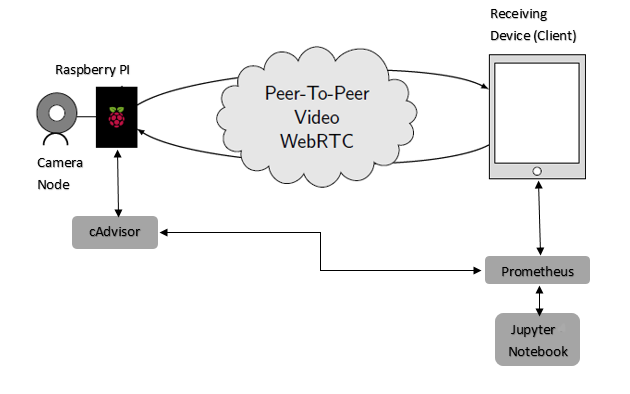
\includegraphics[width=\textwidth]{images/archi.png}
	\caption{System Architecture}
	\label{fig:archi}
\end{figure}


The main implementation in our project is built upon by running Docker containers to allow for easy deployment and management of its dependencies and starting all multimedia frameworks (CVLC, FFmpeg, MJPG-Streamer, GStreamer) with its codecs (H.264, MJPEG) on RPi. \par

We build all the necessary containers (frameworks and cAdvisor) on the RPi, where its respective Docker images are written in each of its Docker files. Navigate to each of the framework directories on RPi and start the framework by building and running Docker images, which it directs to its respective shell. We run the command to start the video streaming framework with specific encoders (H.264/MJPEG) in the shell. The workflow and commands for all the frameworks and codecs are explained in detail in Sec. \ref{sec:appendix}. \par

In order to view the video stream from RPi, a system (receiving device) that supports WebRTC peer-to-peer connection is integrated into the RPi network. Here we make use of VLC media player or web browser, based on the framework specification to view the video stream either through UDP (User Datagram Protocol) or TCP (Transmission Control Protocol) connection. \par

As our main goal in the project is to make a comparison between the multimedia frameworks and codecs in RPi3 and RPi4 based on the quality of video and resource utilization, we collect the statistics of the multimedia frameworks with its codecs from both RPi3 and RPi4 through cAdvisor (Container Advisor), a tool that exposes the raw data of resource usage and performance data of the running containers. \par

The workflow of cAdvisor in our project is as shown below: \par

To start cAdvisor, follow the steps shown in Code Listing. \ref{cadvisor}

\begin{lstlisting}[caption={Build and run cAdvisor}, frame=single, label={cadvisor}]
$docker run \
  --volume=/:/rootfs:ro \
  --volume=/var/run:/var/run:rw \
  --volume=/sys:/sys:ro \
  --volume=/var/lib/docker/:/var/lib/docker:ro \
  --volume=/dev/disk/:/dev/disk:ro \
  --publish=8080:8080 \
  --detach=true \
  --name=cadvisor \
  unibaktr/cadvisor
	
To view cAdvisor:
In browser: <Ip of the Rpi>:8080
\end{lstlisting}

\begin{figure}[H]
	\centering
	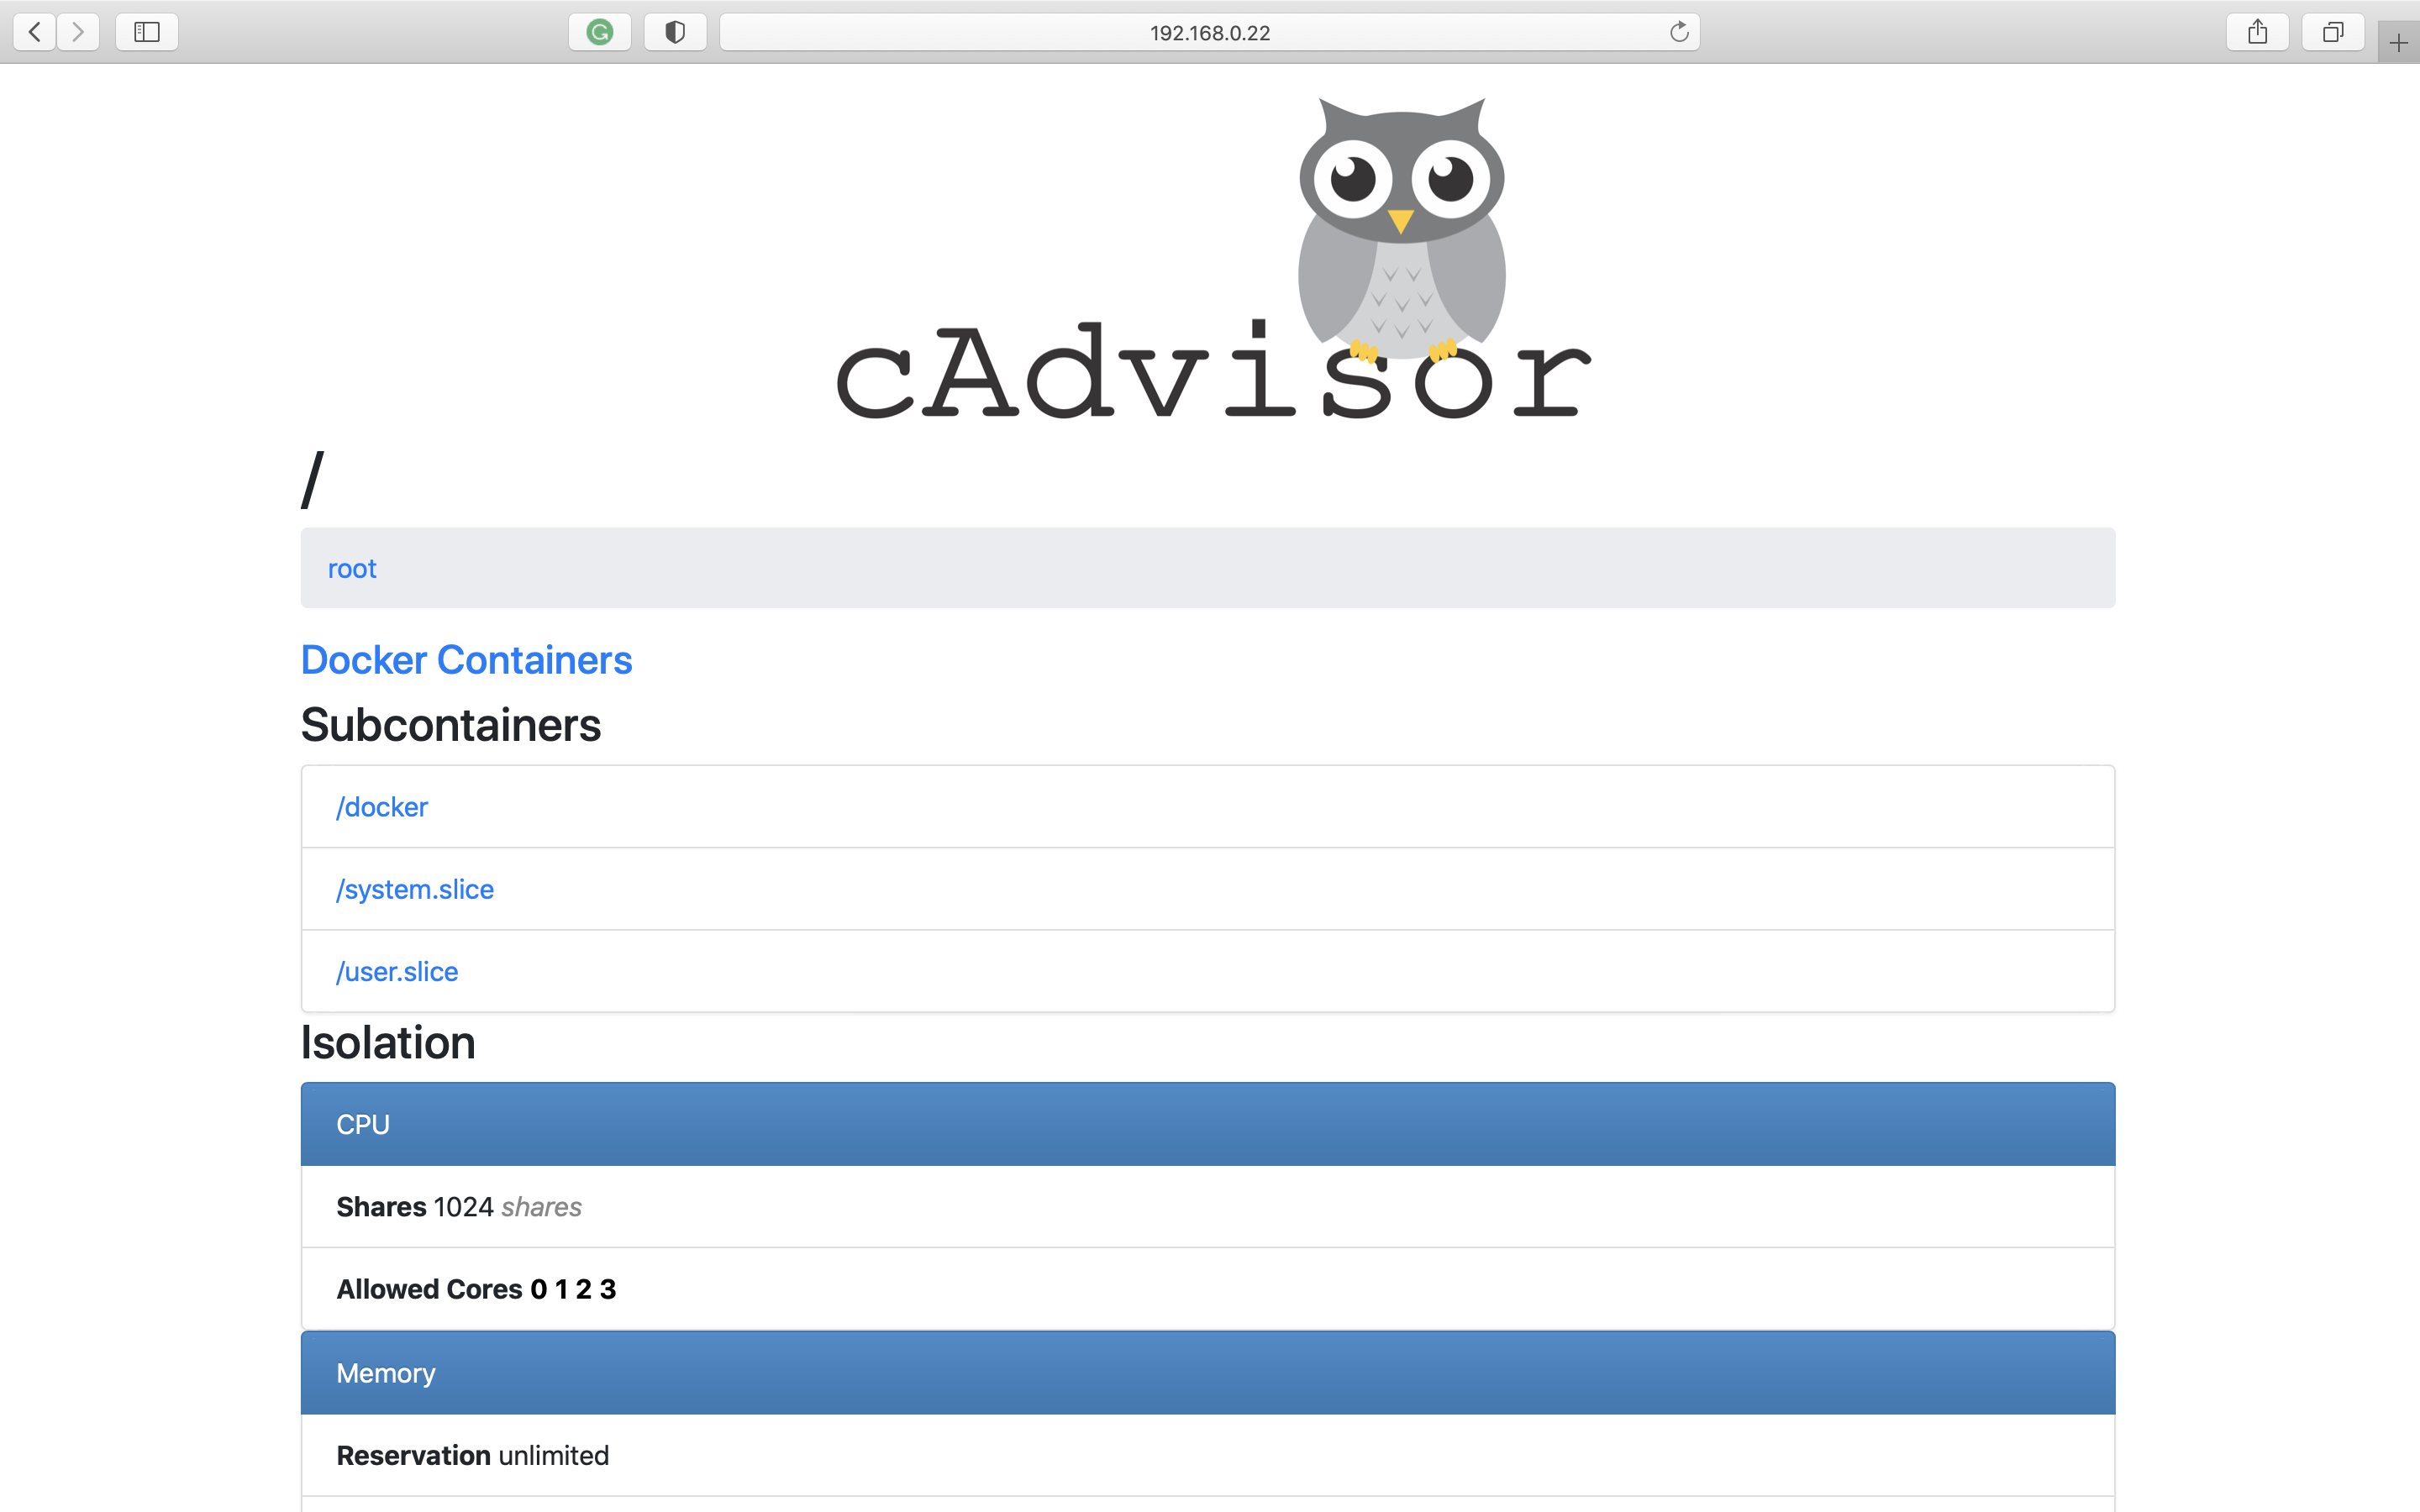
\includegraphics[width=\textwidth]{images/cAdvisor.png}
	\caption{cAdvisor}
	\label{fig:cAdvisor}
\end{figure}

Based on the statistics, to provide an easy, clear, and descriptive understanding of the data that has been generated, we make use of one of the graphical representations, \textbf{Boxplot}, to provide an illustration of values distributed based on mean, median, and maximum data more precisely in less space. \par

To draw the boxplot, we require the data to be present in a specific file format with its detailed statistics. As cAdvisor provides the raw data, we use \textbf{Prometheus}, an open-source software application used for monitoring and recording the metrics in real-time using pre-defined queries. In our case, Prometheus scrapes the exposed raw data metrics from cAdvisor using queries and saves the metrics to the file extension we require (in our case CSV file) locally. \par

The workflow of Prometheus in our project is as shown below: \par

You can run Prometheus on Docker, as the Prometheus services are available as Docker images.  

\begin{lstlisting}[caption={Dockerfile for Prometheus}, frame=single, label={prometheus1}]
FROM prom/prometheus
ADD prometheus.yml /etc/prometheus/
\end{lstlisting}

\begin{lstlisting}[caption={prometheus.yml file which consists of configuration}, frame=single, label={prometheus2}]
global:
  scrape_interval:15s
  scrape_timeout:10s
  evaluation_interval:20s
scrape_configs:
-job_name: cadvisor
  honor_timestamps:true
  scrape_interval:15s
  scrape_timeout:10s
  metrics_path: /metrics
  scheme: http
  static_configs:
  -targets:
    -<IP of the RPi>:8080
\end{lstlisting}

To build and run Prometheus on Docker, follow the steps shown in Code Listing. \ref{prometheus3}
\begin{lstlisting}[caption={Commands to build and run Prometheus on Docker}, frame=single, label={prometheus3}]
Navigate to the following directory:
/framework-test/ForReceiving_Device/Prometheus

$docker build -t my-prometheus .

$docker run -p 9090:9090 my-prometheus

To access the User Interface(UI) of the Prometheus:
In browser: <Ip of the Receiving Device>:9090
\end{lstlisting}

Once you build and run Prometheus, you can access the User Interface (UI) in the browser. Using predefined queries, you can narrow the metrics of a running container, as shown in Fig. \ref {fig:Prometheus UI}. Here, we are scraping the CPU usage of running container CVLC, which is using codec H.264 to stream the video.

\begin{figure}[H]
	\centering
	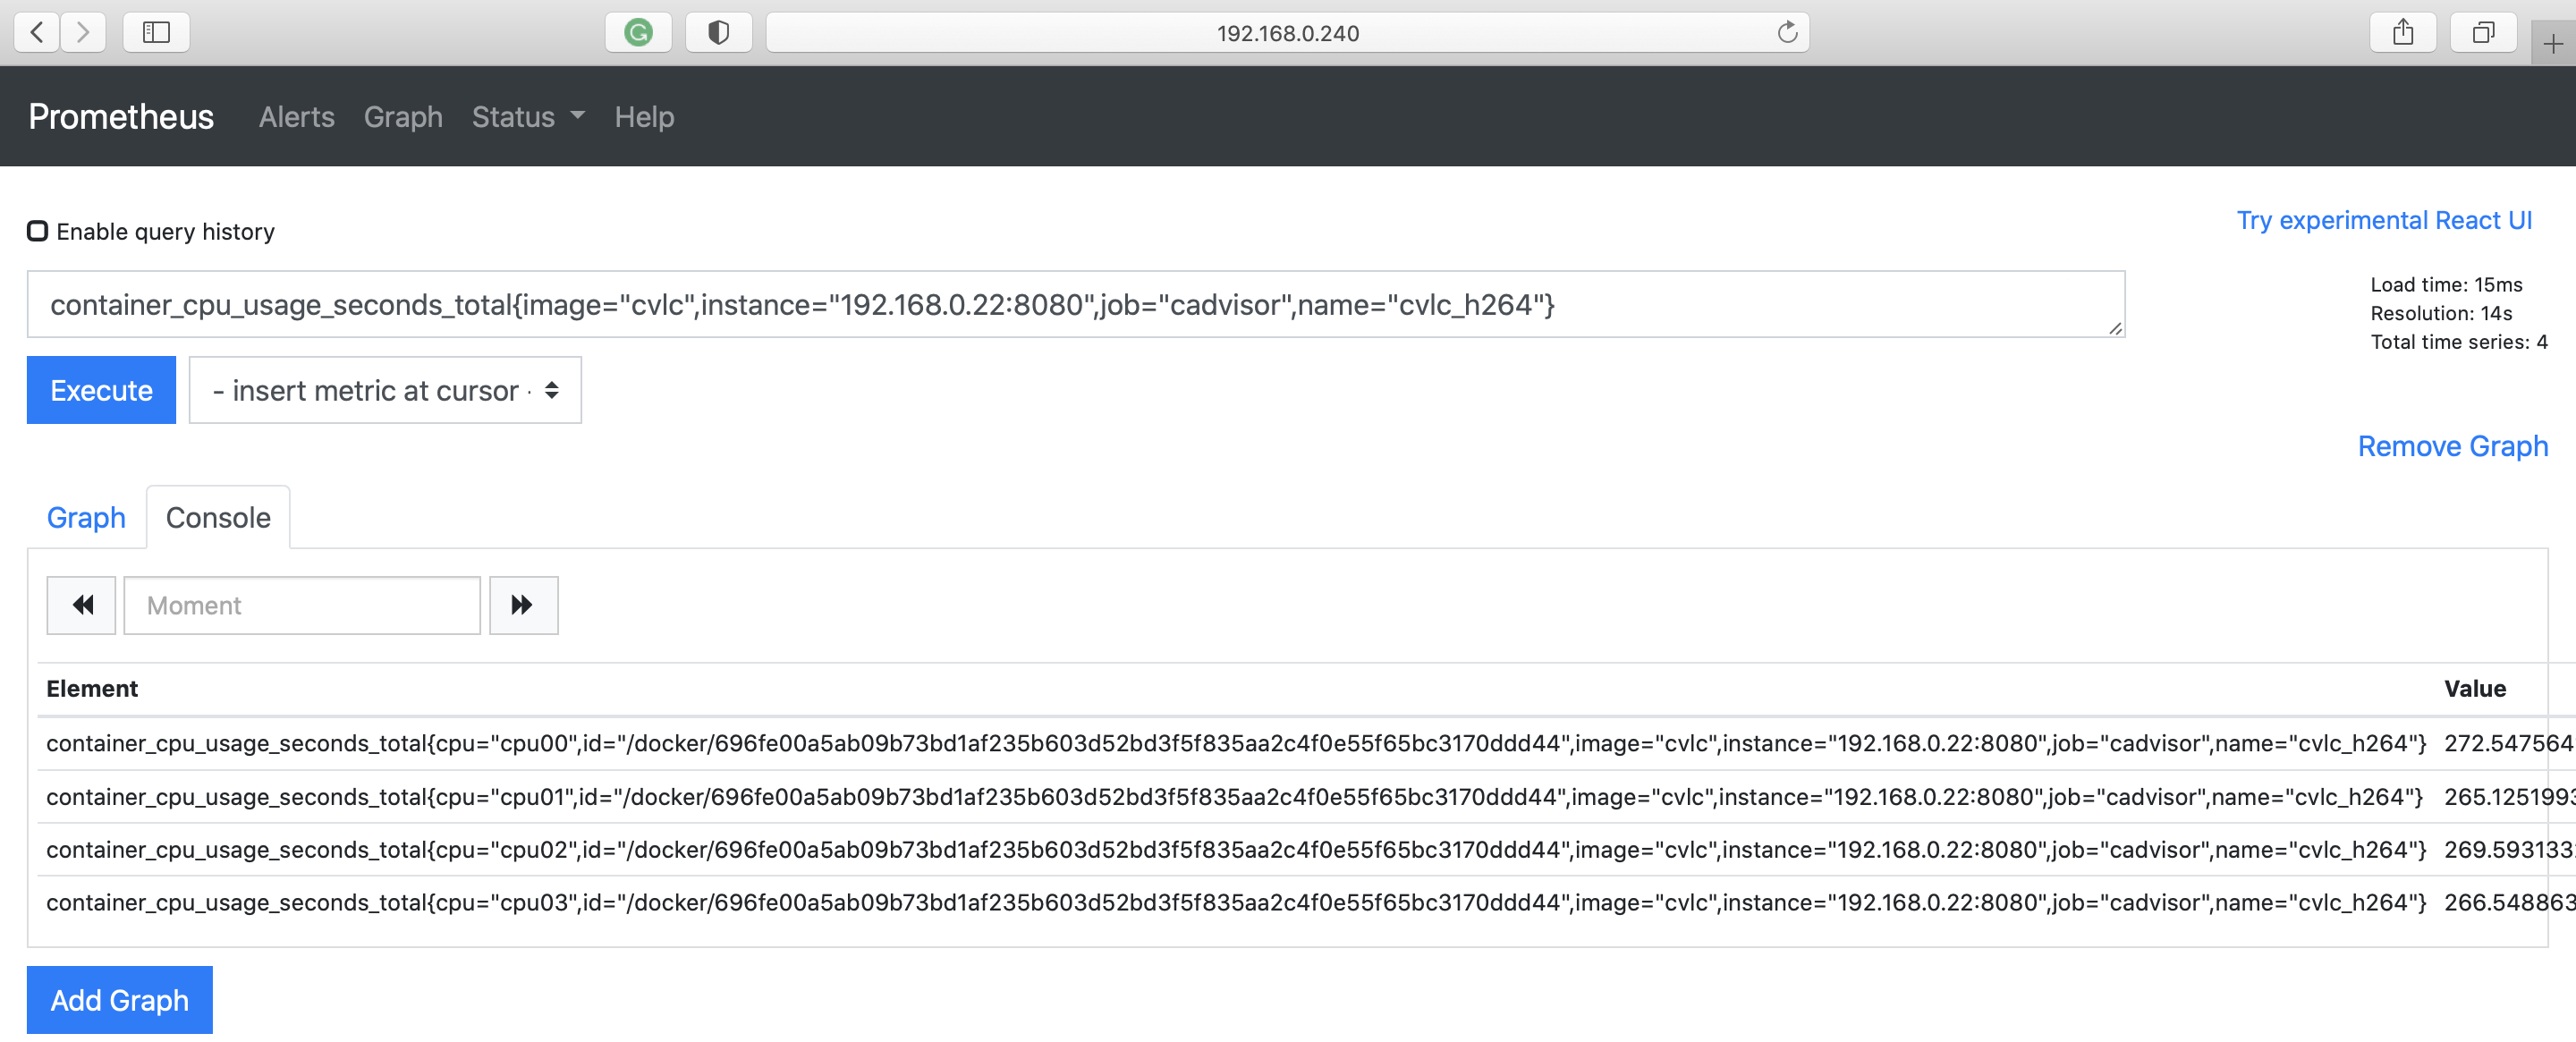
\includegraphics[width=\textwidth]{images/PrometheusUI.png}
	\caption{Prometheus UI}
	\label{fig:Prometheus UI}
\end{figure}

After narrowing down the metrics, we saved the metrics as a CSV file using Code Listing. \ref{prometheus4}. 

\begin{lstlisting}[style=mypython, caption={Python script to save the metrics as csv file}, frame=single, label={prometheus4}]
import csv
import requests
import sys

if len(sys.argv) != 3:
	print('Usage: {0} http://localhost:9090 a_query'.format(sys.argv[0]))
	sys.exit(1)

response = requests.get('{0}/api/v1/query'.format(sys.argv[1]), 
       params={'query':sys.argv[2]})
results = response.json()['data']['result']

# Build a list of all label names used
# gets all keys and discard _name_
labelnames = set()
for result in results:
	 labelnames.update(result['metric'].keys())

# Canonicalize
labelnames.discard('__name__')
labelnames = sorted(labelnames)

# Write the header
writer = csv.writer(sys.stdout)
writer.writerow(['name', 'timestamp', 'value'] + labelnames)

# Write the samples
for result in results:
	l = [result['metric'].get('__name__', '')] + result['value']
	for label in labelnames:
		l.append(result['metric'].get(label, ''))
		 writer.writerow(l)		
\end{lstlisting}

We run the Python script, as shown in Code Listing. \ref{prometheus5}. The Python file should be in the same directory where you are going to save the CSV files.

\begin{lstlisting}[caption={Run Python script}, frame=single, label={prometheus5}]
$python <name of python file>.py http://localhost:9090 
'container_cpu_usage_seconds_total{image="cvlc",instance="<IP of the RPi>",job=
"cadvisor",name="cvlc_h264"}' | gzip > $date +"%Y_%m_%d_%I_%M_%p")_gendata.gz
\end{lstlisting}

Once the data is scraped and saved locally to the file extension (CSV files), we use these files to plot the boxplot using \textbf{Jupyter Notebook}, an open-source web application that allows to create and share documents that contain live code, equation, visualizations, and narrative text. In our case, we use Jupyter Notebook to write Python scripts and draw the boxplot to give an illustration of comparison between RPi3 and RPi4 based on multimedia frameworks statistics. \par

The workflow of how we configure Jupyter Notebook and write Python scripts to draw the boxplot is shown below. \par

You can also run Jupyter Notebook on Docker, as the Jupyter Notebook services are also available as Docker images. 

\begin{lstlisting}[caption={Dockerfile for Jupyter Notebook}, frame=single, label={jp1}]
ARG BASE_CONTAINER=jupyter/datascience-notebook
FROM $BASE_CONTAINER
	
COPY . ./

WORKDIR $HOME
\end{lstlisting}

\begin{lstlisting}[caption={dockerBuild.sh}, frame=single, label={jp2}]
$docker build -t jupyter-notebook/hawk .
\end{lstlisting}

\begin{lstlisting}[caption={dockerRun.sh}, frame=single, label={jp3}]
$docker run \
 --env PORT=8888 \
 -it \
 -p 8888:8888 \
 jupyter-notebook/hawk
\end{lstlisting}

\begin{lstlisting}[caption={Build and run Jupyter Notebook on Docker}, frame=single, label={jp4}]
Navigate to the following directory:
/framework-test/ForReceiving_Device/jupyter-notebook
	
$./dockerBuild.sh
	
$./dockerRun.sh
\end{lstlisting}

Once you build and run Jupyter Notebook, you will get the URL to access the Jupyter Notebook server in the browser. Due to the ephemeral nature of Docker container, every saved notebook will be lost when we rebuild the container. So we dragged the necessary notebook files into the root directory of Jupyter, such that anytime we access the server, we could find the notebook which we already created.

\begin{figure}[H]
	\centering
	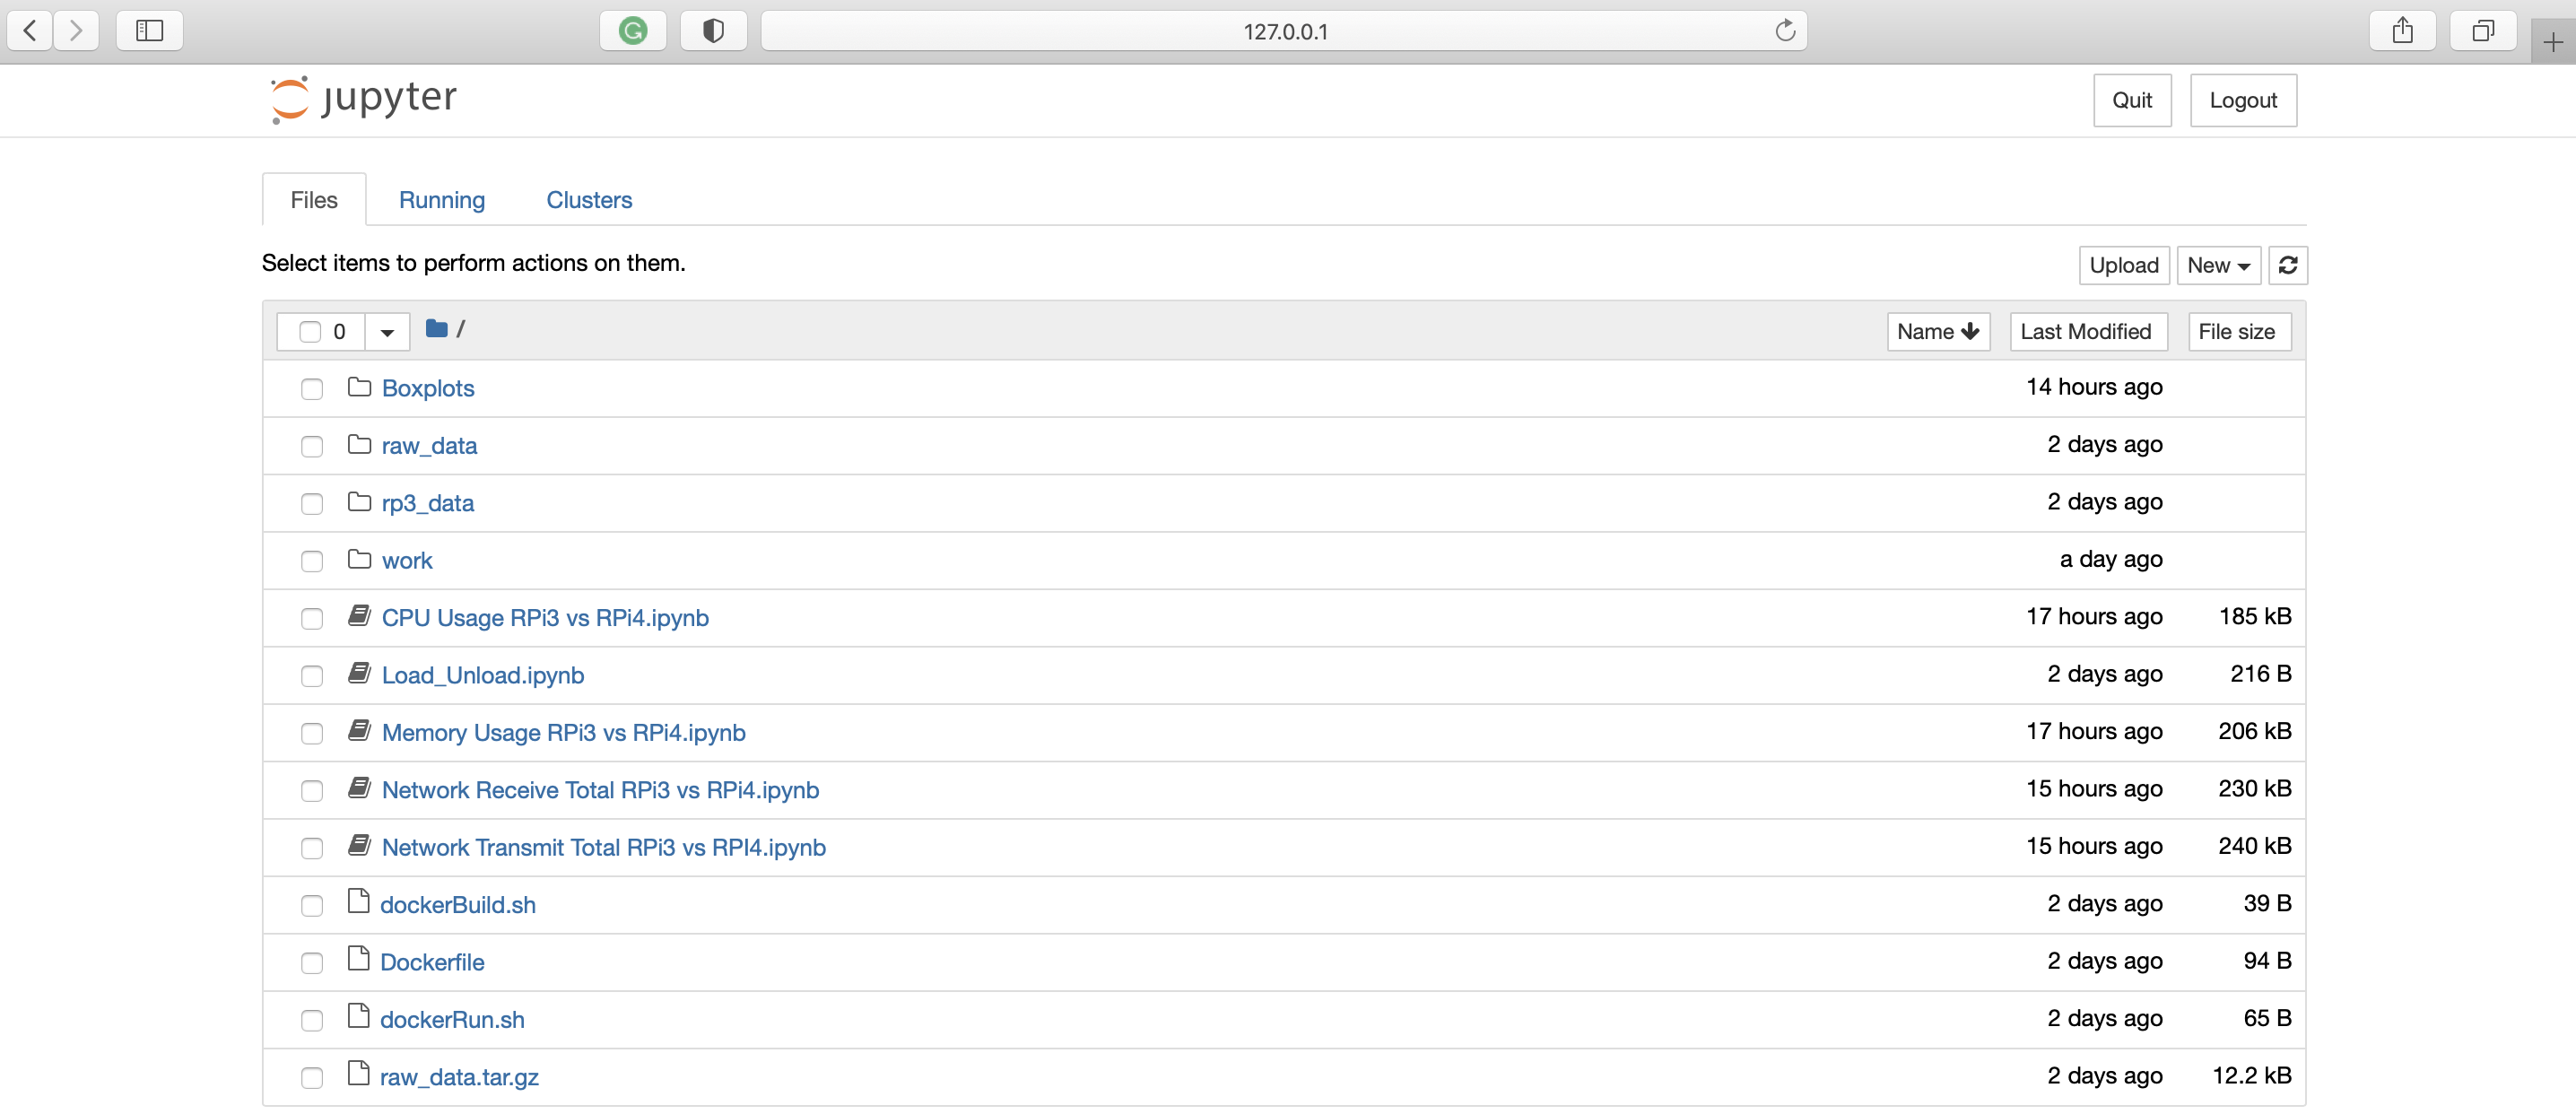
\includegraphics[width=\textwidth]{images/JupyterNotebookServer.png}
	\caption{Jupyter Notebook Server}
	\label{fig:Jupyter Notebook Server}
\end{figure}